% !TEX program = xelatex

\documentclass{resume}
\usepackage{graphicx}
\usepackage{tabu}
\usepackage{multirow}
\usepackage{progressbar}
\usepackage{zh_CN-Adobefonts_external} % Simplified Chinese Support using external fonts (./fonts/zh_CN-Adobe/)
%\usepackage{zh_CN-Adobefonts_internal} % Simplified Chinese Support using system fonts

\begin{document}
\pagenumbering{gobble} % suppress displaying page number

\Large{
  \begin{tabu}{ c l r }
   \multirow{5}{1in}{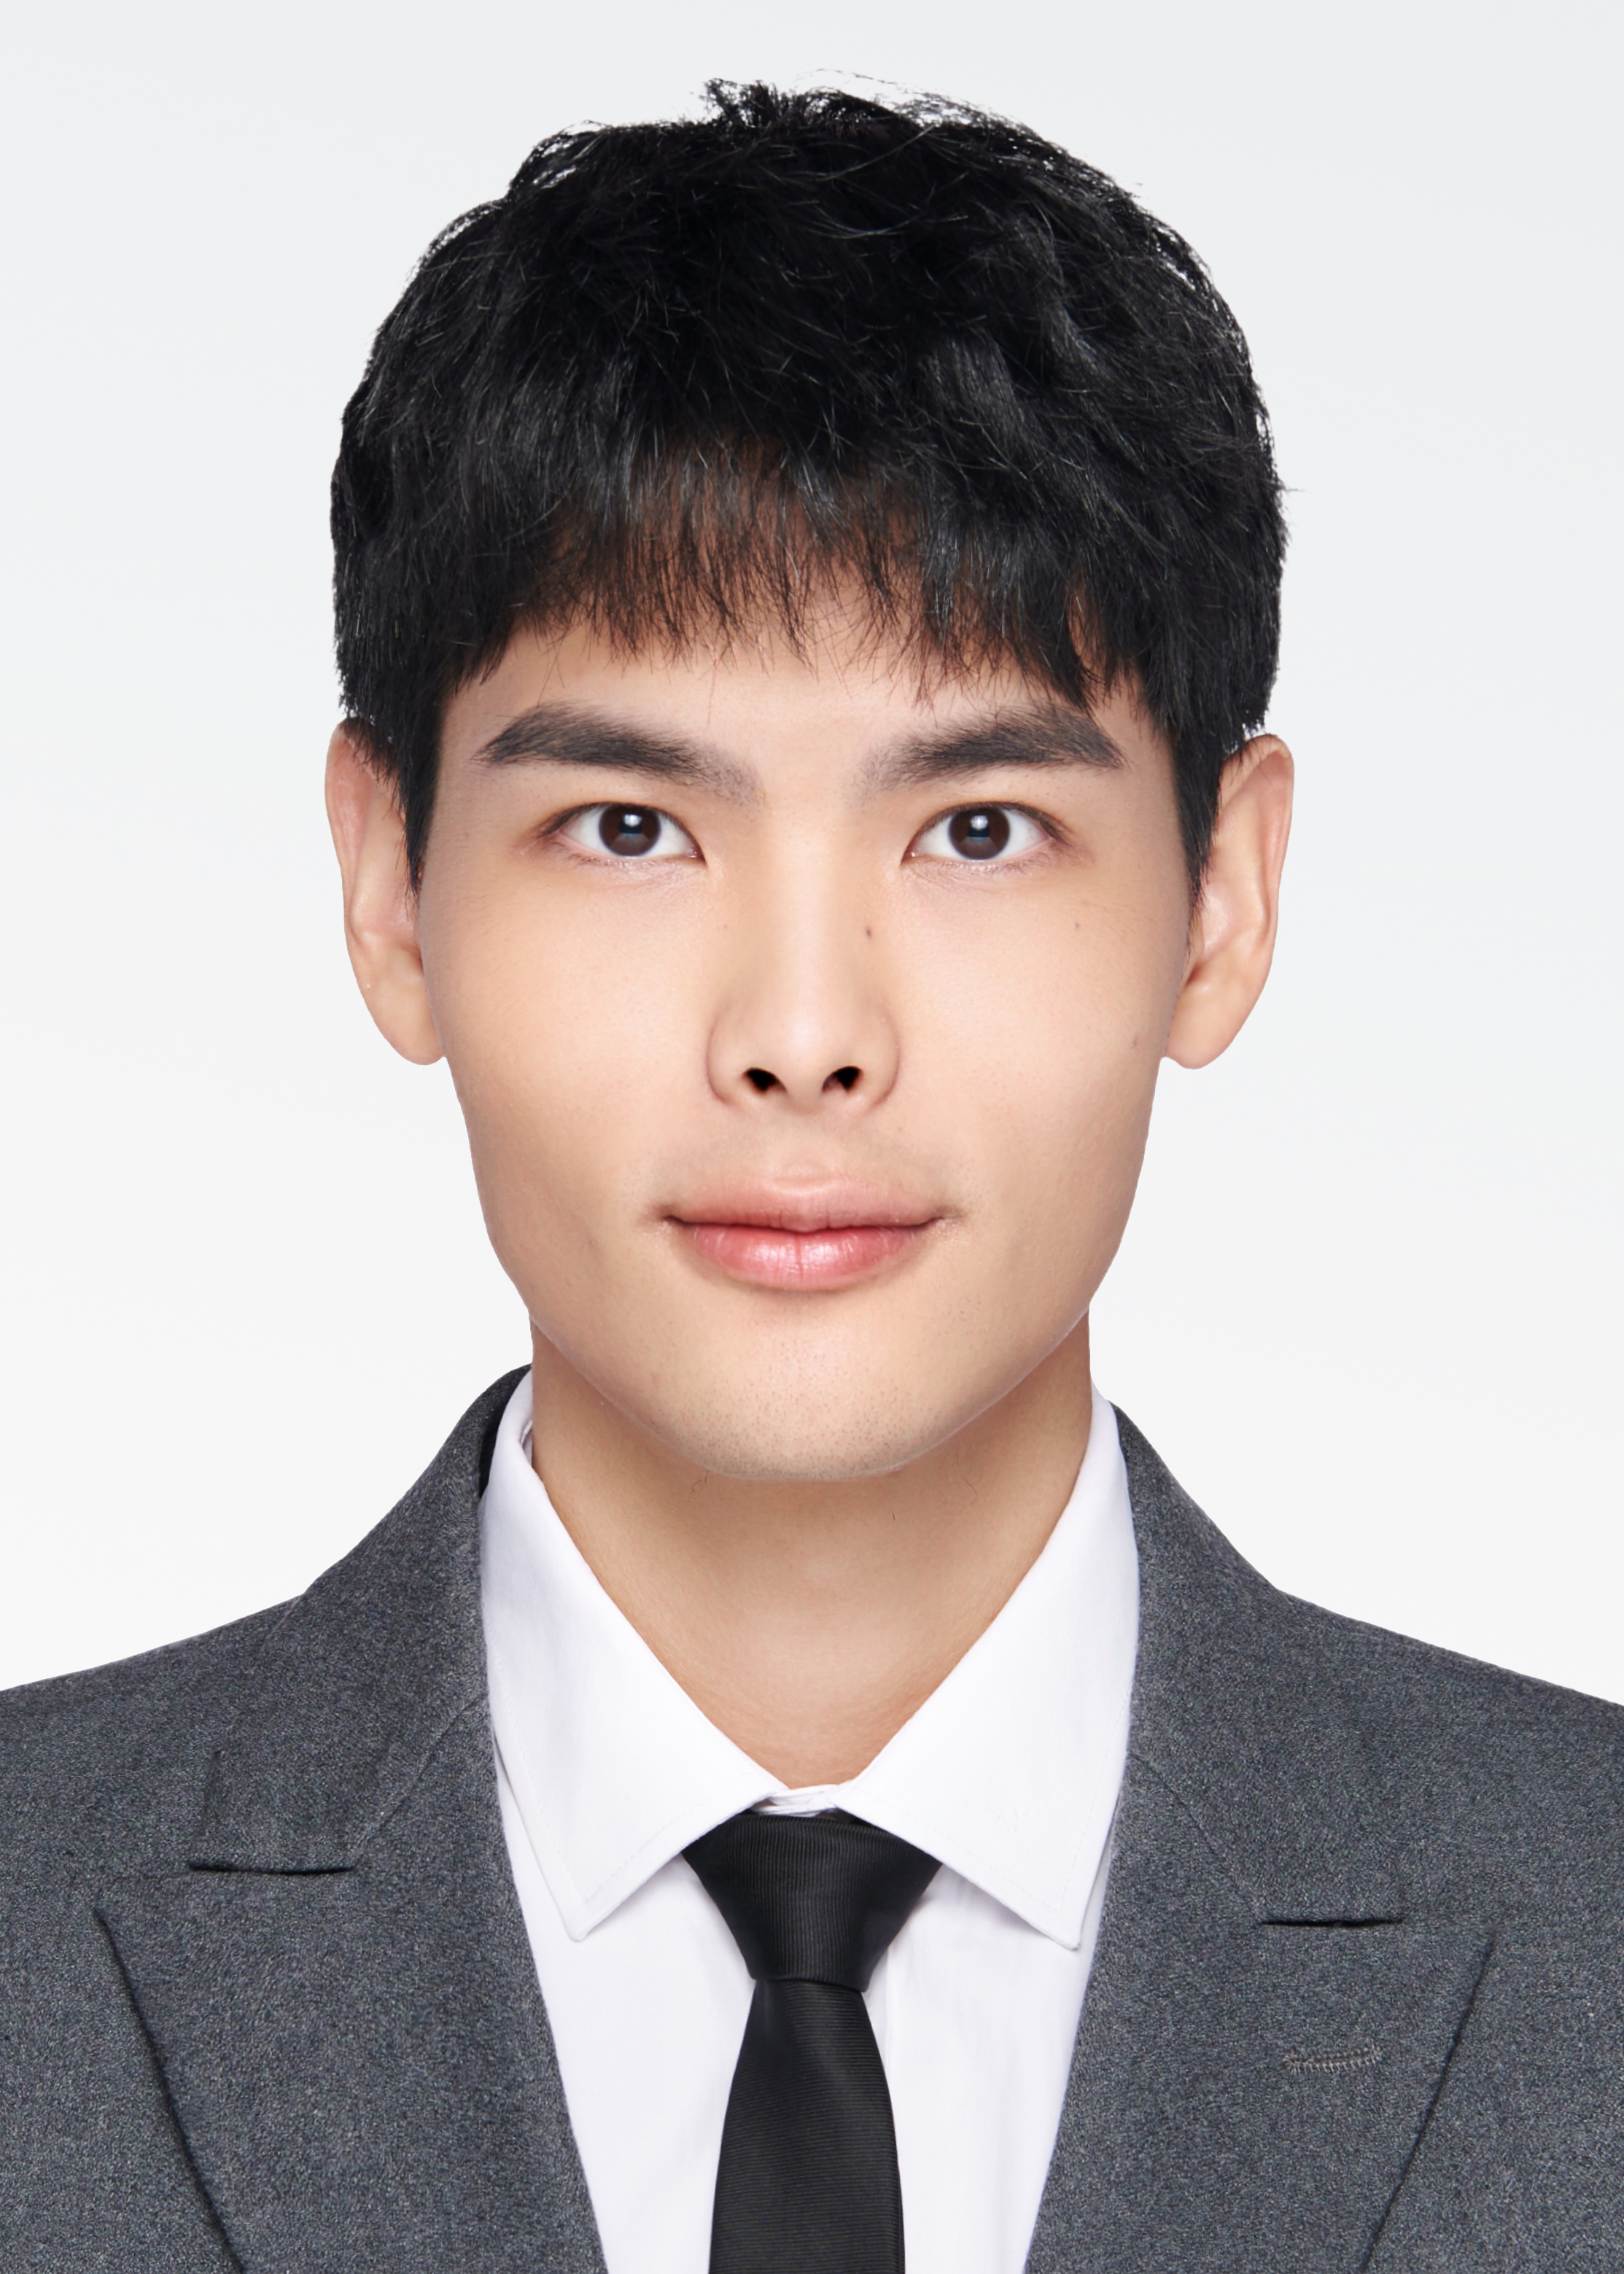
\includegraphics[width=0.88in]{yxh}} & \scshape{Bin Yuan} & {Python~}\progressbar{0.75} \\
    & \email{yuanbin2014@gmail.com} & {Scala~}\progressbar{0.5} \\
    & \phone{(+86) 131-221-87xxx} & {Linux~}\progressbar{0.7} \\
    & \linkedin[billryan8]{https://www.linkedin.com/in/billryan8} & {Flask~}\progressbar{0.5} \\
    & \github[github.com/billryan]{https://github.com/billryan} & {Javascript~}\progressbar{0.5}
  \end{tabu}
}

% \section{\faFileText \ Achievement}
% \begin{itemize}[parsep=0.5ex]
%   \item 政治:65
%   \item 英语一:63
%   \item 数学一:72
%   \item 机械设计基础:73
% \end{itemize}
% \rightline{总分\textit{273分}}
\section{\faThumbsUp \ Self Description}
本人在校成绩优秀、乐观向上,品行端正、自我驱动力强、热爱尝试新事物。本科毕业设计课题为脊柱穿刺机构及其机械臂设计,对机器人设备智能化解决方案有浓厚兴趣。
希望能找到一份与智能制造相关的工作。
\section{\faGraduationCap\  Education}

\datedsubsection{\textbf{河北工业大学},机械设计制造及其自动化,\textit{本科生}}{2018年9月 - 至今}
在校期间完成高等数学、线性代数、概率论、大学物理、大学英 语、控制工程、流体力学等基础学科的学习,完成机械原理、机械设计、机 械制造工程学、机械装备设计以及先进制造技术、互换性与测量 等专业课学习。
\ \textbf{绩点3.17},专业排名前30\%,校二等奖学金(1次),预计2022年6月毕业

\section{\faUsers\ Experience/Project}
\datedsubsection{\textbf{北京精雕(廊坊) |JINGDIAO },实习生}{2021年4月 -- 2021年5月}

于精雕集团实习数控加工中心知识包括:
\begin{itemize}[parsep=0.5ex]
  \item 使用精雕Surfmill软件创建刀具库、在线加工仿真
  \item 零件测量技术与互换性
  \item 机床加工工艺流程,夹具的定位夹紧原理
  \item 工件工艺卡片的制作
\end{itemize}


\datedsubsection{\textbf{工程训练比赛},队长,\textit{智能配送无人机赛项}}{2021年3月 -- 2021年4月}

为团队做出如下贡献:
\begin{itemize}[parsep=0.5ex]
  \item 参与并主导无人机动力系统设计并进行参数调整
  \item 参与构思设计机械投放装置实现小体积精准快速投放
  \item 飞控自动化运行程序编写,将ADRC抗扰算法应用于无人机姿态控制
  \item 无人机整体三维模型绘制
\end{itemize}




% Reference Test
%\datedsubsection{\textbf{Paper Title\cite{zaharia2012resilient}}}{May. 2015}
%An xxx optimized for xxx\cite{verma2015large}
%\begin{itemize}
%  \item main contribution
%\end{itemize}

\section{\faCogs\ Skills}
% increase linespacing [parsep=0.5ex]
\begin{itemize}[parsep=0.5ex]
  \item 建模水平:SolidWorks曲面建模;AutoCAD
  \item 计算机水平:Office,计算机二级C语言,\LaTeX,设计软件PS、AE、Pr、Ai,仿真软件MultiPhysics
  \item 英语水平:通过CET-6(\textit{453分}),具有良好听说读写能力
\end{itemize}

\section{\faTrophy\ Honors and Awards}
\datedline{\textit{第三名},河北省大学生运动会男子四百米,\textit{二级运动员}}{2019 年7 月}
\datedline{\textit{第二名},天津市大学生运动会男子四百米栏}{2021年10月}
\datedline{\textit{第三名},全国大学生工程训练大赛智能配送无人机赛项河北赛区}{2021年4月}



%% Reference
%\newpage
%\bibliographystyle{IEEETran}
%\bibliography{mycite}
\end{document}
